\documentclass[a4paper, 12pt]{paper}

\usepackage[portuges]{babel}
\usepackage[utf8]{inputenc}
\usepackage{amsmath}
\usepackage{indentfirst}
\usepackage{blindtext}
\usepackage{graphicx}
\usepackage[hyphens]{url}
\usepackage[hidelinks]{hyperref}
\usepackage{gensymb}
\usepackage[top=2cm, bottom=2cm, left=3cm, right=2cm]{geometry}
\usepackage[table]{xcolor}
\usepackage{pbox}
\usepackage{wrapfig}
\usepackage{pdflscape}
\usepackage{longtable}

\setlength{\parindent}{3em}
\setlength{\parskip}{0.4em}

\renewcommand{\UrlFont}{\scriptsize}
\author{I. Messina, I. Abreu, P. Gil, R. Bellotti, T. Proux}

\title{Plano de Negócios - eVarsity}
\begin{document}
    \begin{titlepage}
    	\begin{minipage}[c][3cm][c]{3cm}
    		
\includegraphics[height=3cm]{img/ufrj_logo.png}
    	\end{minipage}
    	\begin{minipage}[c][3cm][c]{10cm}
    		Universidade Federal do Rio de Janeiro \\
    		Organização das Indústrias \\
    		Plano de Negócios
    	\end{minipage}
    	\begin{center}
    		\vspace{95pt}

    		\huge{Plano de Negócios - eVarsity}
    		\vspace{260pt}
    	\end{center}

    	\begin{center}
            Ian Messina \\
            Igor Abreu\\
            Pedro Gil\\
            Rafael Bellotti\\
            Thasus Proux\\
    	\end{center}

    	\begin{center}
    		\vspace{\fill}
    		Rio de Janeiro, 24 de Novembro de 2016
    	\end{center}
    \end{titlepage}
\newpage
\tableofcontents
\listoffigures
\newpage

\section{Plano de Gestão}
\subsection{Fatores Culturais}


Com os grandes avanços que ocorreram na área de tecnologia da informação nas últimas décadas, especialmente a partir da virada do milênio, os equipamentos eletrônicos estão cada vez mais presentes nos cotidianos individuais, e têm ressignificando múltiplas formas de interação entre as pessoas. As crianças nascidas neste período têm entrado em contato com computadores pessoais, consoles de videogame, tablets e smartphones cada vez mais cedo. Um dos maiores atrativos para essas gerações, ao longo de todas essas plataformas, são os jogos eletrônicos.

Por sua vez, a crescente capacidade computacional dos computadores permite a criação de jogos com complexidade crescente, apresentando desde gráficos extremamente elaborados, passando por mecânicas simplificadas de jogo através de controles por movimento, até narrativas profundas e complexas, capazes de atrair consumidores de idade mais avançada, ou interessados em elementos estéticos e literários.

Esse crescimento do escopo da produção de jogos eletrônicos, então, tem gerado um enorme crescimento dessa indústria. O mercado de jogos eletrônicos está mundialmente em ascensão e deve gerar US\$99,6 bilhões até o final do ano, se consolidando como o maior ramo da indústria do entretenimento, ultrapassando o cinema. Este valor é 8.5\% maior que o do mesmo período no ano passado. A Newzoo, empresa que realizou a pesquisa, também prevê um crescimento positivo no Brasil: considerado o décimo primeiro país com maior mercado de jogos no mundo. Além disso, os dados da pesquisa apontam que dos 33,6 milhões de usuários brasileiros, 56\% investem dinheiro em jogos.

Não é apenas através do consumo e da utilização desses jogos eletrônicos, porém, que se desenvolvem atividades. O ato de jogar se tornou, por si só, entretenimento. Jogar por diversão se tornou uma ferramenta para produção de conteúdo de distribuição online que, hoje, se consolidou como uma das maiores indústrias do entretenimento online, através de plataformas de compartilhamento de vídeo e de livestreaming como o YouTube e a Twitch. Os produtores de conteúdo focado em jogos eletrônicos representam a maior fatia de arrecadação em relação ao conjunto dos produtores independentes - os grandes canais promovidos por gigantes da mídia tradicional, como VEVO, não são aqui contabilizados.

Não é só diversão que atrai público, porém. Uma enorme indústria vem se consolidando ao longo da última década e meia, baseada em eventos que envolvem jogos eletrônicos com caráter competitivo: os esportes eletrônicos, ou eSports. Os principais títulos competitivos atuais apresentam múltiplos torneios por ano, com premiações que podem chegar à casa das dezenas de milhões de dólares\footnote{\url{http://www.pcgamer.com/dota-2-international-2016-breaks-own-prize-pool-record-now-biggest-in-esports-history/}} e com milhões de espectadores simultâneos. Empresas de mídia tradicional, apercebendo-se da tendência de crescimento da área, já se fazem presentes nesse cenário. A MTG (Modern Times Group), um conglomerado sueco de mídia e dono da ESL (Electronic Sports League) e da Dreamhack (espécie de Campus Party de proporções maiores) é um dos maiores players da indústria. A TBS (Turner Broadcast System), um dos principais canais de televisão dos EUA e propriedade da Time Warner, um dos maiores conglomerados de mídia do mundo, produz campeonatos de esportes eletrônicos para a televisão aberta norte-americana, e seu próximo evento, a ser realizado em Janeiro de 2016, apresentará 1 milhão de dólares em premiações\footnote{\url{http://www.eleague.com/major/}}. Estima-se que o número de pessoas que reconheçam os esportes eletrônicos tenha passado de 1 bilhão e que o número de espectadores tenha ultrapassado os 300 milhões\footnote{\url{https://newzoo.com/insights/articles/global-esports-awareness-exceeds-1-billion-as-new-initiatives-launched/}}.

\begin{figure}[!ht]
	\centering
	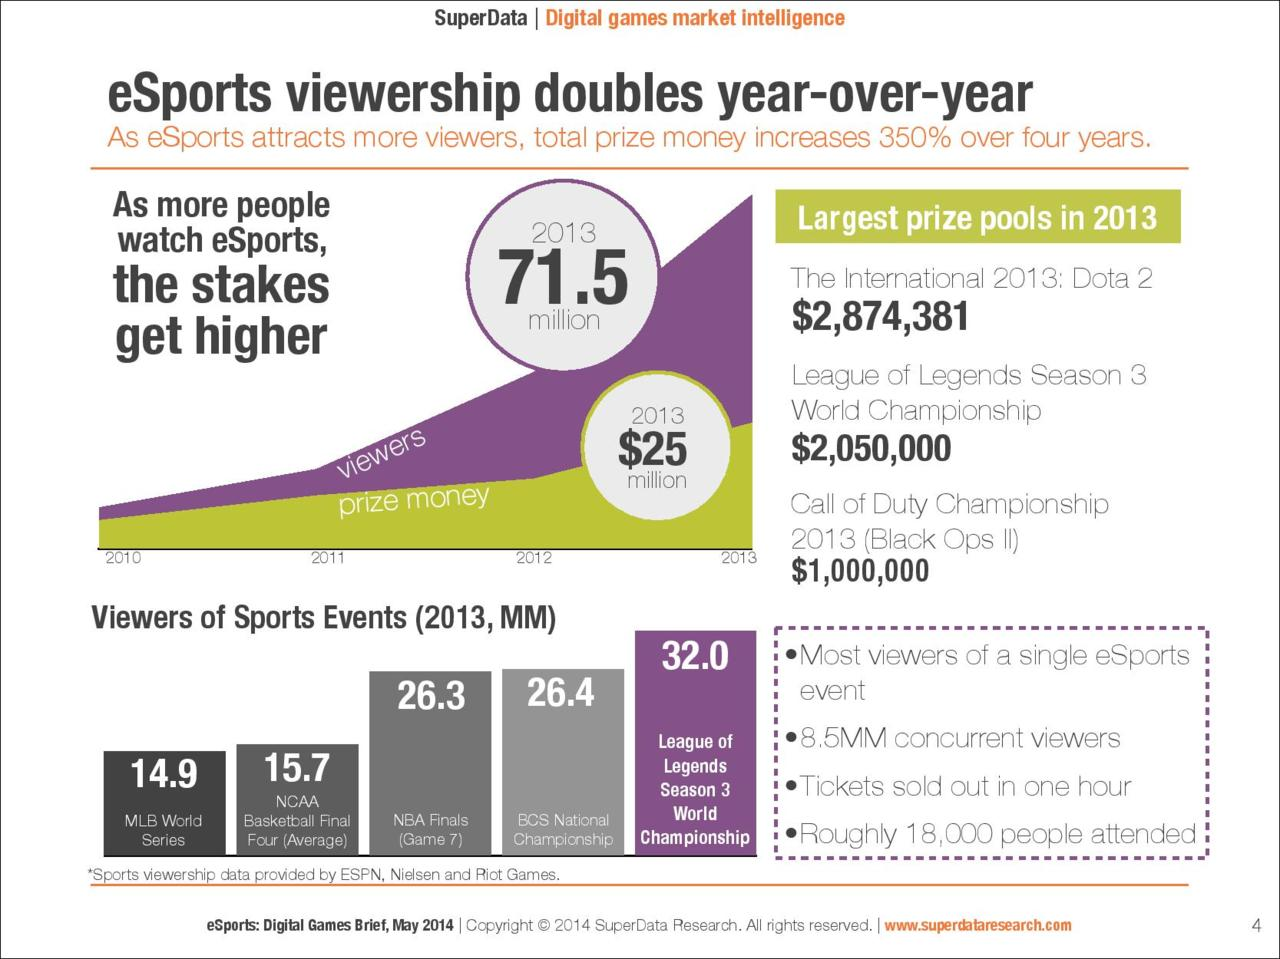
\includegraphics[scale=0.45]{img/img01.png}
	\caption{Crescimento do número de Telespectadores de eSport}
\end{figure}

Essa tendência de crescimento da audiência - e da formação de jogadores competitivos - é igualmente encontrada no Brasil, que configura na lista dos 10 países que mais assistem conteúdo deste tipo. Um dos principais times e bicampeão mundial em 2016 de um dos títulos mais assistidos de eSports, Counter-Strike:Global Offensive, é formado exclusivamente por jogadores brasileiros. O conjunto de 5 jogadores já faturarou mais de 1 milhão de dólares em premiações e, sob a organização alemã SKGaming, recebe U\$10.000,00 de salário mensal por jogador. Jogadores brasileiros de League of Legends, como Felipe “brTT” Gonçalves\footnote{\url{http://sportv.globo.com/site/games/noticia/2016/11/jogador-brasileiro-mais-famoso-de-lol-felie-brtt-deixa-pain-gaming.html}} e Gabriel “Kami” Bohn\footnote{\url{http://sportv.globo.com/sit e/games/noticia/2016/07/gabriel-kami-o-jovem-fenomeno-do-lol-no-brasil-que-vale-r-1-milhao.html}}, por suas vezes, figuram entre os 10 jogadores de eSports com maior número de seguidores no mundo.

\begin{figure}[!ht]
	\centering
	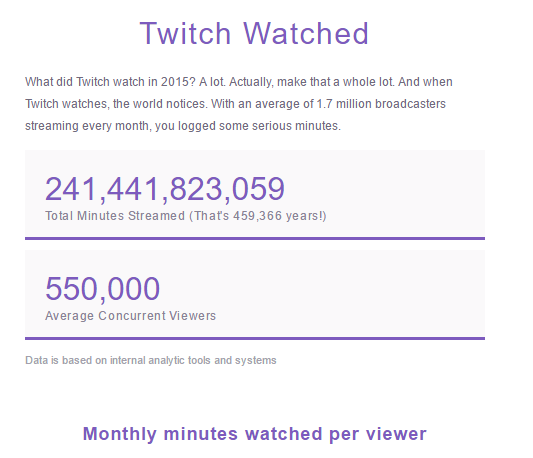
\includegraphics[scale=1]{img/img02.png}
	\caption{Dados sobre a plataforma de Streaming da Twitch}
\end{figure}
É possível afirmar que existe, então, um mercado consumidor bastante significativo no Brasil, tanto de jogadores quanto de espectadores de esportes eletrônicos. Um mercado, porém, ainda muito pouco explorado. A grande maioria dos eventos e produtoras internacionais de real importância quase nunca puseram os pés no país, relegando torneios de nível mais baixo para aqui serem sediados. Também, o cenário nacional de eSports se mostra bastante amador e incipiente, ainda. Os produtores locais, assim como as organizações de jogadores e os times nacionais que não se mudaram para outros continentes, possuem pouca influência internacional e pequenas capitalizações. O cenário local de eSports é praticamente intocado por grandes empreendimentos, ou mesmo por empreendimentos de caráter verdadeiramente profissional. Em suma, o mercado de eSports no Brasil é fértil e pouquíssimo explorado.
\subsection{Fatores Ambientais}
Os eventos serão separados em etapas online e presenciais. As etapas online não apresentam diretamente nenhum impacto ambiental, pois seu conteúdo está atrelado ao meio virtual. Os eventos presenciais apresentam risco de poluição sonora; porém, poderiam ser sediados em lugares propriamente aparelhados com proteção acústica projetada, podendo abaixar esse risco até que seja considerado nulo.
\subsection{Fatores Mercadológicos}
Três tipos de consumidor devem ser levados em conta. É considerado um consumidor em potencial do primeiro tipo todos que possuem um computador conectado à rede e que tenham interesse por jogos eletrônicos e estejam interessados em participar ou assistir os jogos. Os consumidores do segundo tipo são clientes que desejam contratar serviços de consultoria para ajudar a planejar eventos de jogos competitivos. Os do terceiro tipo são empresas que busquem oferecer patrocínio a eventos de esportes eletrônicos em troca da divulga\c{c}\~{a}o de suas marcas e de outros \textit{payoffs}. A seguir será realizado uma análise dos principais agentes no mercado de jogos eletrônicos.
\subsubsection{Serviços de Streaming}
Serviços de streaming como YouTube e Twitch influenciam fortemente o mercado de jogos. Por se tratar das plataformas de acompanhamento de jogos em tempo real mais fortes no mercado, se torna indispensável considerar seus efeitos no mercado de jogos.

De acordo com a plataforma Twitch, a média de espectadores simultâneos é de 550 mil e o número de minutos médios que cada espectador assiste usando a plataforma Twitch é de 421,6 por mês, já na plataforma YouTube foram 291 minutos por mês. O gráfico abaixo mostra o crescimento do número de espectadores e canais entre dia 20 de junho de 2012 e dia 29 de outubro de 2016 na plataforma Twitch.
\begin{figure}[!ht]
	\centering
	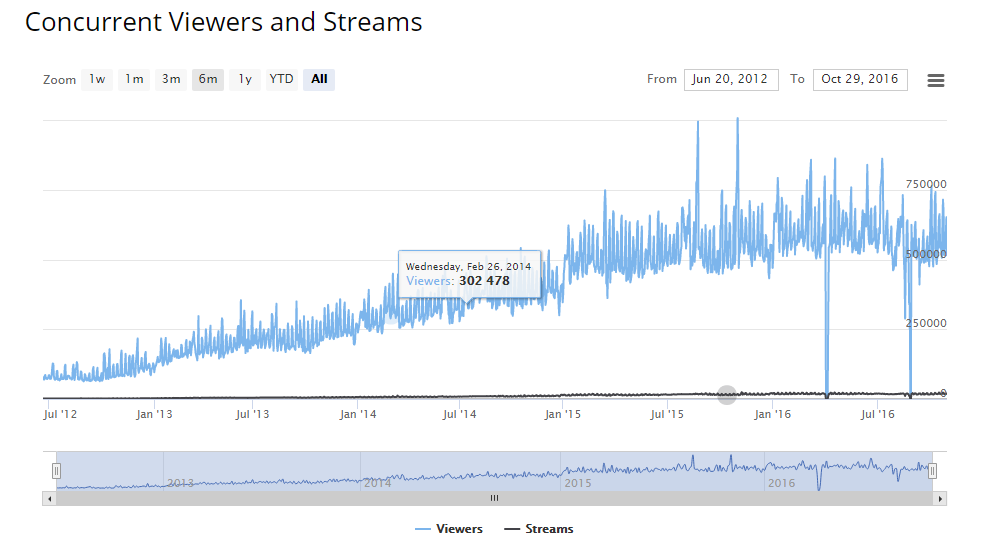
\includegraphics[scale=0.62]{img/img03.png}
	\caption{Aumento do número de telespectadores na plataforma de Streaming da Twitch}
\end{figure}
\subsubsection{Eventos Presenciais}
Eventos de competição presenciais reúnem espectadores e competidores em um único espaço, onde os primeiros têm a oportunidade de observar os jogadores competindo. As empresas que criam os jogos tendem a dar reconhecimento a tais eventos e costumam ajudar na divulgação deles em suas páginas web e nas áreas de notícias dentro do portal de seus jogos.

Para exemplificar com números, o IEM Katowice, realizado em Fevereiro de 2016, teve mais de 104 mil espectadores somente no evento, ou seja, sem contar com os espectadores que assistiam por meio da televisão ou plataformas de streaming.

O The International 2016, maior campeonato de Dota 2 do ano, que teve mais de 17 mil pessoas simultaneamente em um estádio, chegou a uma premiação de U\$20.770.460, o maior valor de premiação da história dos eSports - e maior do que a premiação de alguns dos maiores eventos esportivos do mundo, como o Superbowl \footnote{\url{http://www.polygon.com/2014/7/19/5918845/dota-2-international-2014-champions-money-winners}}. Desse valor, somente U\$1.600.000,00 vieram da empresa Valve, criadora do jogo e responsável pela organização do evento; todo o resto foi obtido via ferramentas de financiamento coletivo, direto dos espectadores do evento.
\subsubsection{Televisão}
Embora ainda tenham pouco impacto no mundo da transmissão por televisão, os eSports estão crescendo nesse tipo de mídia. Atualmente, canais de grande nome, como CNN, TBS e ESPN, no caso internacional, e SporTV e Esporte Interativo no caso nacional, estão cada vez mais investindo em jogos eletrônicos para atrair mais espectadores para seus canais de televisão\footnote{\url{http://esporteinterativo.com.br/esports/eleague-chega-aos-canais-esporte-interativo-e-reacende-a-paixao-do-brasil-por-counter-strike/}}\footnote{\url{http://sportv.globo.com/site/noticia/2016/04/sportv-inova-e-transmite-ao-vivo-torneio-do-game-dota-2.html}}. Além disso, a empresa ESL anunciou um canal de televisão dedicado a jogos eletrônicos chamado de esportsTV.
\subsection{Fatores Geográficos}
Os eventos puramente online não apresentam nenhuma barreira geográfica, mas são passíveis de gerar barreiras para usuários de regiões com acesso limitado à internet. Por outro lado, os eventos presenciais requerem que os espectadores estejam no evento fisicamente. Isto acaba gerando uma forte barreira geográfica, pois somente pessoas nativas ao local de realização do evento, ou com condições financeiras favoráveis para bancar os custos de viagens, hospedagem e do evento em si, além de possuírem tempo disponível, poderão participar dos eventos.
\subsection{Fatores Econômicos}
A economia do país está apresentando resultados surpreendentes com os poucos eventos que foram organizados. São Paulo sediou nos dias 28 a 30 de outubro de 2016 a quarta edição do torneio de CS:GO Pro League, premiando o primeiro colocado com US\$200.000, sendo as premiações totais somadas equivalentes a US\$750.000. O Ginásio do Ibirapuera foi completamente  tomado, com todos os ingressos, para todos os dias do evento, tendo sido vendidos. A audiência online ultrapassou 100.000 espectadores simultâneos nos momentos de pico.

Outro grande fator é o crescimento do poder de compra da população brasileira em relação ao período inicial de desenvolvimento dos eSports, há mais de uma década atrás. Mesmo com os impactos do presente momento de instabilidade econômica pelo qual passa o país, é possível afirmar que a disponibilidade de renda média da população brasileira para consumo de jogos eletrônicos - e, indiretamente, de produtos ligados aos eSports - é maior. Junte-se a isso o fato de que os preços dos jogos estão cada vez mais acessíveis, por conta do advento da distribuição digital, que reduz os custos de distribuição ao fornecer o download direto dos jogos via internet, e é possível afirmar que existe um grande potencial econômico para o desenvolvimento deste cenário.

Deve-se também levar em conta que as plataformas de transmissão por meio digital são abertas de forma gratuita a qualquer um que tenha acesso a internet. Dessa forma, qualquer um que possa acessar os sites pode acompanhar os jogos e campeonatos, de forma que a barreira de entrada para espectadores é muito pequena.
\subsection{Fatores Sociais}
Uma grande parcela dos interessados nessas modalidades são jovens-adultos - muitos universitários - e adolescentes, embora a demografia esteja se expandindo em ambas as direções do espectro. É considerado de vital importância, então,  não somente planejar eventos pensando nos calendários acadêmicos, como também oferecer opções baratas de pacotes que cubram menos atividades durante o evento, mas que permitam a jovens com recursos financeiros limitados assistirem aos jogos.
\subsection{Fatores Tecnológicos}
O projeto é inteiramente baseado em tecnologia. Tanto os eventos presenciais quanto os online são construídos em cima de competições realizadas em computadores e via infraestrutura de rede e hospedagem de servidores. Não apenas a competição em si, porém, mas também todo o mecanismo de cobertura e de transmissão das partidas, tanto \textit{in loco} quanto via internet, são realizados através de meios digitais.

Para realização de eventos online, é necessária infraestrutura remota de hospedagem em servidores para a conexão dos jogadores à partida e um sistema para observação e transmissão do jogo via livestream, assim como mecanismos de pós-produção para realizar as transições entre as diferentes telas (composição dos times, estatísticas, etc.).


\begin{wrapfigure}{l}{5.5cm}
    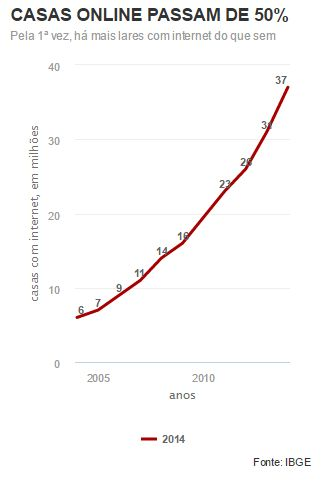
\includegraphics[scale=0.5]{img/img04.png}
    \caption{Casas com acesso \`{a} internet}
\end{wrapfigure}

Para realização de eventos \textit{in loco}, é necessária infraestrutura presencial de hospedagem de servidores próprios para conexão dos jogadores à partida e o mesmo sistema para observação e transmissão, também com pós-produção. Neste caso, além da pós-produção do conteúdo diretamente relacionado ao jogo, existe a possibilidade da existência de câmeras filmando o evento em tempo real, o que implica na necessidade de produção e filtragem de canais simultâneos de imagens ao vivo, assim como de iluminação e estudo de captação de áudio.
No campo da produção posterior de conteúdo em cima dos eventos, é necessária estrutura para captura de vídeo e de som direto dos jogos, em alta definição e fidelidade, assim como para captação de vídeos do ambiente do evento em alta qualidade, com boa iluminação e captação de som.

Excedendo-se o caráter da produção e direcionando o foco para o consumo,disso, é fundamental que o espectador que não esteja \textit{in loco} possua acesso à internet. O IBGE publicou, através da PNAD de 2011, dados que mostram que o acesso a internet cresceu para todas as camadas sociais do país. Isto se deve, provavelmente, a melhorias no mercado de trabalho e na renda pessoal, além de expansão da área de cobertura e melhoria da infraestrutura existente, o que implicou na redução de custos para contratação deste tipo de serviço.

Os dados do IBGE referentes a 2014 mostram que 36,8 milhões de domicílios estavam conectadas à internet, representando um total de 54,9\% da população brasileira. Tal índice é consideravelmente maior que o de 2013 (48\%), mostrando crescimento considerável desse segmento.

Além disso, o IBGE indicou que a quantidade de internautas chegou a 54,4\% das pessoas com mais de 10 anos em 2014. São 95,4 milhões de brasileiros com acesso a internet. Essa dupla ultrapassagem vem de uma mudança de metodologia do IBGE. Apenas as conexões feitas com computador eram registradas até a PNAD de 2013; a partir daí, o instituto passou a contabilizar acessos com smartphones, tablets, TVs e outros dispositivos, todos passíveis de ser utilizados como meios de acompanhar o cenário competitivo de esportes eletrônicos.

Além disso, de acordo com dados da Wikipedia, de 2012, o Brasil atualmente se encontra em quarto no ranking dos países que possuem o maior número absoluto de pessoas com acesso a internet.

\begin{figure}[!ht]
    \centering
    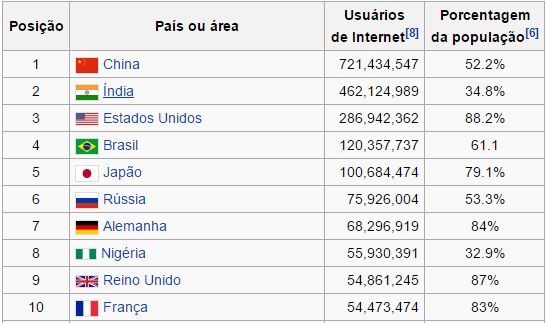
\includegraphics[scale=0.5]{img/img05.png}
    \caption{Us\'{u}arios de internet por pa\'{i}ses}
\end{figure}

\newpage

\begin{landscape}
\subsection{Análise SWOT}
    \begin{figure}[!ht]
        \centering
        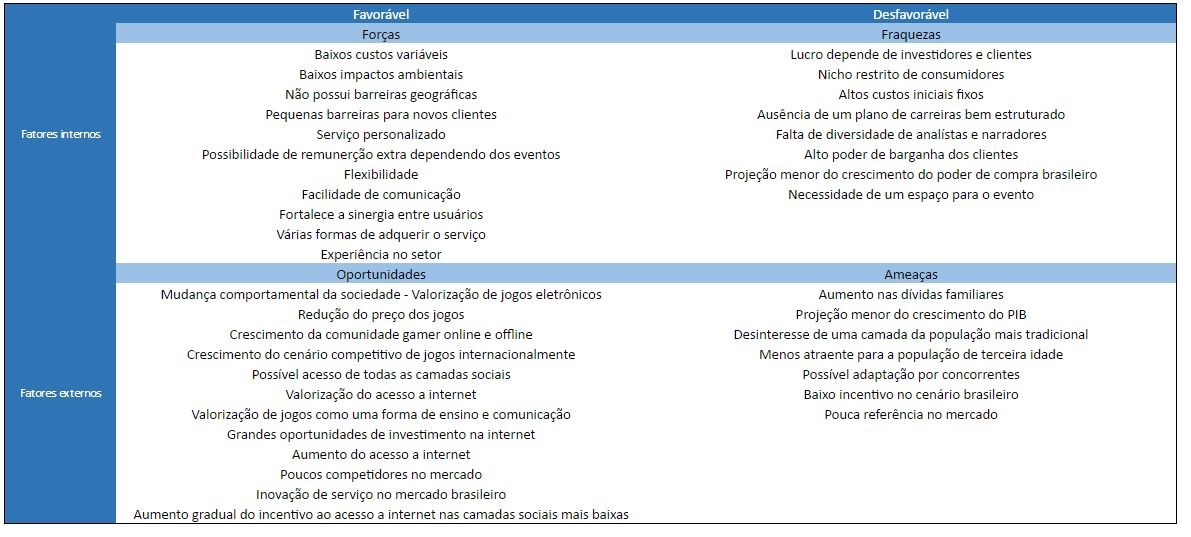
\includegraphics[width=25cm,height=12cm]{img/img06.png}
        \caption{Análise SWOT}
    \end{figure}
\newpage
\subsection{Modelo de Negócio Canvas}
\begin{figure}[!ht]
    \centering
    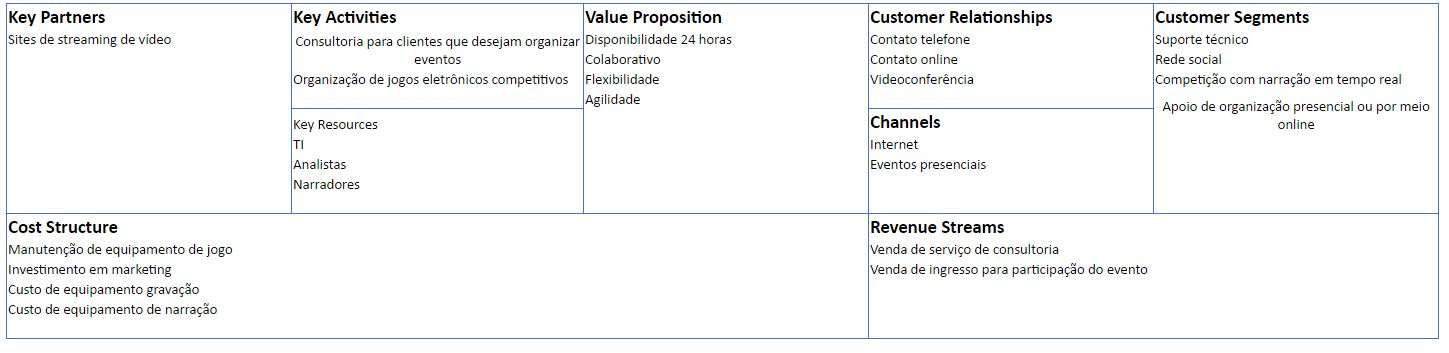
\includegraphics[width=25cm,height=10cm]{img/img07.png}
    \caption{Modelo Canvas}
\end{figure}
\newpage
\subsection{Fatores Críticos de sucesso}
\begin{figure}[!ht]
    \centering
    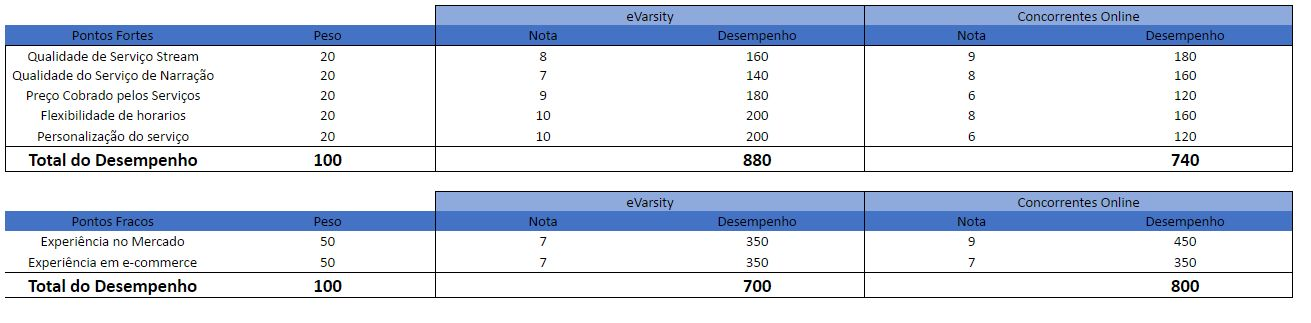
\includegraphics[scale=0.56]{img/img08.png}
    \caption{Posicionamento Competitivo}
\end{figure}
Ao examinar o posicionamento competitivo da eVarsity, ao interpretar os números encontrados na análise dos pontos fortes da empresa, é fácil perceber o diferencial da empresa em relação aos concorrentes.  Porém, em relação aos pontos fracos, existe clara desvantagem no que se refere aos possíveis concorrentes. Isso, porém, é apenas uma maneira de ilustrar a divisão clara entre o nicho de mercado a ser afetado pela eVarsity, composto principalmente pelo cenário amador/semi-profissional Universitário e acadêmico, e o nicho focal de seus concorrentes, composto pelo cenário “profissional”. A eVarsity, embora possua concorrentes gerais, não possui nenhum concorrente direto. Mesmo que afetando um mesmo mercado geral, os nichos específicos não se mostram concorrentes.
\end{landscape}



\newpage
\section{Plano de Marketing}
\subsection{Descrição dos Serviços}
eVarsity é uma empresa da área do entretenimento, oferecendo serviços que contém, mas não se limitam exclusivamente, a organização de eventos presenciais e não-presenciais de eSport e espaços de divulgação de marcas e empresas.
\subsection{Forças do Marketing}
\subsubsection{Produto}
Os produtos oferecidos pela eVarsity podem ser classificados em duas classes: serviços B2C (business to commerce - empresa para consumidor) e serviços B2B (business to business - empresa para empresa).

Na classe de serviço B2C, a atividade é a organização direta dos campeonatos. Isso engloba o fornecimento de toda a infraestrutura necessária para os eventos. Nos campeonatos não-presenciais, servidores para os jogos que necessitem ser hospedados e uma equipe para divulgar e narrar as partidas.

Já para os campeonatos presenciais, além do espaço físico preparado para acomodar os torcedores e as equipes, também é necessário servidores, além de computadores que serão fornecidos aos participantes, com teclados e mouses disponíveis caso necessário (a maioria das equipes preferem levar seus próprios periféricos para as competições).

Na classe de serviço B2B, existem dois produtos. O primeiro, a atividade de consultoria para a organização de eventos, prestando serviços para outras empresas. Nessa situação, nosso papel dependeria do que a empresa necessitaria baseado nos requisitos expostos nos parágrafos acima. O segundo, o oferecimento de espaço de divulgação para empresas que se interessem em se fazer presentes no espaço universitário, e a coleta de dados dos espectadores do evento para compor os bancos de dados de \textit{headhunter} destas mesmas empresas.
\subsubsection{Preço}
Definir um preço para as atividades da eVarsity esbarra na variabilidade que pode existir de acordo com o serviço que a empresa oferecer. Para as duas classes de serviços oferecidos, o consumidor pode variar entre empresas de variados tamanhos e diferentes consumidores finais, influenciando diretamente a definição do preço. Além disso, dependendo da dimensão e da duração do evento, assim como do espaço físico onde será realizado e das requisições específicas de momento, é possível a existência de métricas distintas e momentâneas para precificação dos serviços prestados.

Em suma, objetivo de nossa organização é que nossos serviços adicionem valor aos nossos clientes e o preço será proporcional a esse valor.

A organização de eventos universitários e amadores/semi-profissionais cumpre duas demandas pouco cobertas pela concorrência. A primeira, promover a valorização de potenciais esportistas eletrônicos através da realização de eventos que servem de validação prática de suas eventuais profissões, promovendo sua continuidade e crescimento no cenário local e fomentando o crescimento de seus espaços de divulgação pessoal nas mídias sociais. A segunda, fornecer um meio para que os fãs desses esportes possam assistir torneios presenciais de qualidade e estarem constantemente antenados às mais recentes novidades no cenário local de eSports.

Consideramos que organizar um campeonato tem grande valor:

1 - aos jogadores, pois permite que demonstrem suas habilidades a seus (possíveis) fãs e potenciais empregadores;

2 - a outras equipes (que possam estar a procura de membros);

3 - a empresas e organizações: tanto patrocinadores, que têm na audiência deste tipo de torneio universitário a atenção de jovens qualificados/se qualificando para o mercado de trabalho; quanto contratantes, que passam a conseguir viabilizar um serviço que, de outra forma, não seria possível, até mesmo pela ausência de empresas similares.

Assim, entende-se como justa a premissa de monetizar as três esferas de potenciais clientes sob o alcance da eVarsity, tendo em vista os benefícios gerados a todos e os gastos inerentes à produção dos campeonatos. Porém, também entende-se que a função social da eVarsity se mostra maior do que apenas investimento e geração de renda, por encadear no desenvolvimento de todo um cenário social e econômico ainda pouco representado no país.

Segue, portanto, um pequeno resumo do potencial de precificação dos serviços oferecidos pela eVarsity, no que considera cada um dos tipos de consumidor final:

\textbf{Para a audiência:}

Para eventos não-presenciais, acredita-se que o valor imediato dos eventos não seja tão grande, dada a distância entre o espectador e o torneio e os custos menores de produção. Isso torna não muito interessante a cobrança de uma taxa, especialmente no que toca a dificuldade - e os gastos -  tecnológica de restringir a audiência via Internet. Porém, pensamos em produzir um material exclusivo a longo prazo, fornecido apenas para assinantes. Igualmente, a existência de uma loja online de produtos da eVarsity ajudar na capitalização de ganhos para a empresa.

Para eventos presenciais, o valor despendido é maior, o que justificaria a cobrança de uma taxa de entrada para os espectadores. Porém, considerando-se a pouca disponibilidade direta de renda do público universitário para gastos supérfluos, imagina-se que a cobrança de taxas, pelo menos a curto prazo, não resultaria proveitosa. A venda de merchandising \textit{in loco} e a capitalização da audiência como ferramenta de barganha para com possíveis patrocinadores dos eventos se mostram alternativas de capitalização mais viáveis.

Estima-se que um valor médio de R\$15,00 por peça de merchandising a ser vendida (considerando-se itens caros, como camisas, e baratos, como pins) seja interessante para atrair a atenção de múltiplos espectadores.

\textbf{Para os Jogadores:}

Tanto para eventos online, quanto para eventos \textit{in loco}, é definida a cobrança de uma taxa de inscrição devida à existência de premiação em dinheiro para os vencedores. Competições com premiação, na visão tradicional da indústria, exigem algum tipo de retorno por parte dos jogadores. Nos grandes cenários internacionais, os grandes times pagam com suas próprias imagens e presença, capazes de atrair espectadores. Nos menores cenários, como o atingido pela eVarsity, os times pagam valores simbólicos de inscrição.

Os valores de inscrição variam de acordo com as dimensões do torneio e com o tamanho do montante para premiação, mas experiências anteriores provam que um valor de R\$10,00 por integrante é considerado baixo. Para o curto prazo, ainda na fase de consolidação da empresa, cobrar um valor que orbite o supracitado é ideal.

\textbf{Para as Empresas:}

Para as empresas patrocinadoras, o valor total do patrocínio dependerá do alcance da coleta de dados do evento e do número de espectadores diretos ou indiretos a serem afetados pelas ações de divulgação da eVarsity. Estimar um preço padrão por patrocínio, portanto, se mostra exercício complexo. Experiências anteriores, porém, parecem dizer que os patrocinadores, no presente momento, dispõe-se a bancar um preço de R\$18,00 por espectador afetado, em média. A curto prazo, estimar valores de cobrança próximos a este é o ideal. A longo prazo, porém, com o aumento da penetrabilidade da eVarsity no mercado e com a consolidação de sua marca, não há motivos para n\~{a}o revisar este valor para cima.

Para as empresas contratantes de consultoria, seguimos a estratégia de preço pelo valor adicionado ao cliente. Nessa direção, a cobrança de valor para a outra empresa seria complementar as necessidades para a organização do evento. Por exemplo, entre uma empresa que, por si, forneça os computadores e o espaço físico, e outra que não os forneça, existirá uma discrepância de preço. A precificação precisa, tabelada, sugerida para as atividades de curto prazo da eVarsity se encontram na seção \ref{servcons}.

\subsubsection{Praça}
O principal canal de distribuição dos eventos será a Internet. Existem diversas plataformas e comunidades online para a transmissão de competições, inclusive em tempo real. A longo prazo, é possível a elaboração de um site próprio. Os eventos online serão realizados todos remotamente, via internet. Os eventos presenciais ocorrerão em universidades e escritórios alugados/comprados pela organização. Tanto online quanto \textit{in loco}, contarão com narração em tempo real e também com cobertura de streaming para audiência.

A atividade de consultoria poderá ser realizada em espaços cedidos pelas empresas contratantes ou em espaços oferecidos pela própria eVarsity, obtidos em caráter perene ou através de locação.
\subsubsection{Promoção}
A atividade promocional da eVarsity tem como objetivo prioritário promover o conhecimento, por parte de seu potencial mercado consumidor, dos serviços oferecidos. Considerando-se a proximidade de nossas atividades e de nosso mercado consumidor com a internet e as redes sociais, faz-se claro que a alternativa de divulgação mais efetiva, especialmente no que se considera alcance e custo, é através da Internet e via Mídias Sociais. A própria pulverização de nosso potencial mercado consumidor, assumidamente capaz de assistir e participar das atividades (mesmo que apenas das online) à distância, faz toda e qualquer divulgação física e localizada muito menos efetiva. Desta forma, atividades promocionais tradicionais, com a utilização de mídias físicas, só serão postas em prática em situações específicas, especialmente na proximidade das localidades - e no período de tempo de ocorrência - onde serão realizadas as atividades presenciais, ou em localizações focais de nosso mercado consumidor (o Centro de Tecnologia da UFRJ, ou o Campus da Praia Vermelha da UFF, por exemplo).
\subsubsection{Pessoas}
Uma descrição detalhada da equipe será apresentada na seção \ref{layoutop} deste documento. Uma descrição branda resumiria as pessoas envolvidas na empresa nas seguintes categorias:

1- Diretores: responsáveis pela organização e pela viabilização técnica e financeira de eventos, além de integrarem o conselho gestor e de planejamento estratégico da eVarsity;

2 - Narradores, Observadores e Comentaristas: responsáveis por descrever e explicar o que ocorre durante os jogos;

3 - Equipe Técnica: responsáveis pela criação e manutenção da infraestrutura tecnológica, informacional e logística da eVarsity e de suas atividades, e pela confecção direta do material de divulgação.
\subsubsection{Processos}
Os processos operacionais podem-se dividir em duas áreas: organização de evento próprio ou organização de evento para terceiros.

Em um evento próprio, o comitê de planejamento se reunirá e definirá as datas, fazendo assim um calendário anual com todos os eventos organizados pela empresa. O planejamento de cada evento deve conter todas as informações necessárias para sua organização - presencial ou não, número de participantes, premiação e outros.

Em um evento organizado para terceiros, o comitê de planejamento oferecerá um projeto descritivo para o contratante, informando os custos e necessidades para a realização de um evento com o padrão solicitado e a divulgação e a realização será executada seguindo o mesmo modelo de organização própria.
\newpage
\section{Plano Operacional}
\subsection{Layout Operacional}
\label{layoutop}
A organização utilizará as principais plataformas sociais para divulgar seu trabalho; a equipe de comunicação e marketing será responsável por mantê-los. Nossa principal mídia de divulgação será uma página própria no Facebook. Nesta página divulgaremos streams na Twitch e no Youtube, bem como campeonatos e eventos. Contaremos também, se necessário, com um servidor do Discord para entrar em contato com nossa comunidade de uma forma mais interativa. O Twitter será uma plataforma de divulgação em paralelo ao Facebook. Teremos também, em segundo plano, um sub-Reddit.

A principal idéia é aproveitar as plataformas sociais já existente com o objetivo de reduzir custos de hospedagem e alcançar o público que já as utiliza. O website site contará com links para as principais rede sociais e cadastro de eventos tanto por partes do jogador, como por parte do espectador, se necessário.
\subsection{Capacidade de Prestação}
Para campeonatos presenciais, sem jogos simultâneos, estima-se que serão necessários 10 computadores com as seguintes configurações recomendadas:

Windows 7, Core I5,  6Gb de Ram, 30 Gb de HD, Monitor Full HD 23’’, Placa de Video NVIDIA GTX 760.

Os periféricos (mouses, teclados e headsets) são trazidos pelos próprios competidores, por questão de adaptação pessoal e preferência própria constatada nos jogadores. Além dos hardwares informados, para campeonatos presenciais deveremos contar com 10 abafadores de som.

Para campeonatos online, a maioria dos jogos atendidos pela  organização oferece uma infraestrutura de salas privadas para a criação dos nossos torneios, permitindo uma maior flexibilidade e um custo quase nulo para a organização. Para jogos que necessitem de uma infraestrutura própria, contaremos com um servidor que hospedará os jogos, tanto no caso presencial, quanto no caso online (se for necessário).

É importante lembrar que para campeonatos presenciais, ocorrerá uma limitação física de espaço para o número de telespectadores no local, entretanto embora o evento seja presencial, os jogos continuarão sendo transmitidos através dos canais de streaming.
\subsection{Processos Operacionais}
Os processos operacionais podem se dividir em duas áreas: organização de evento próprio ou organização de evento para terceiros.

\begin{figure}[!ht]
    \centering
    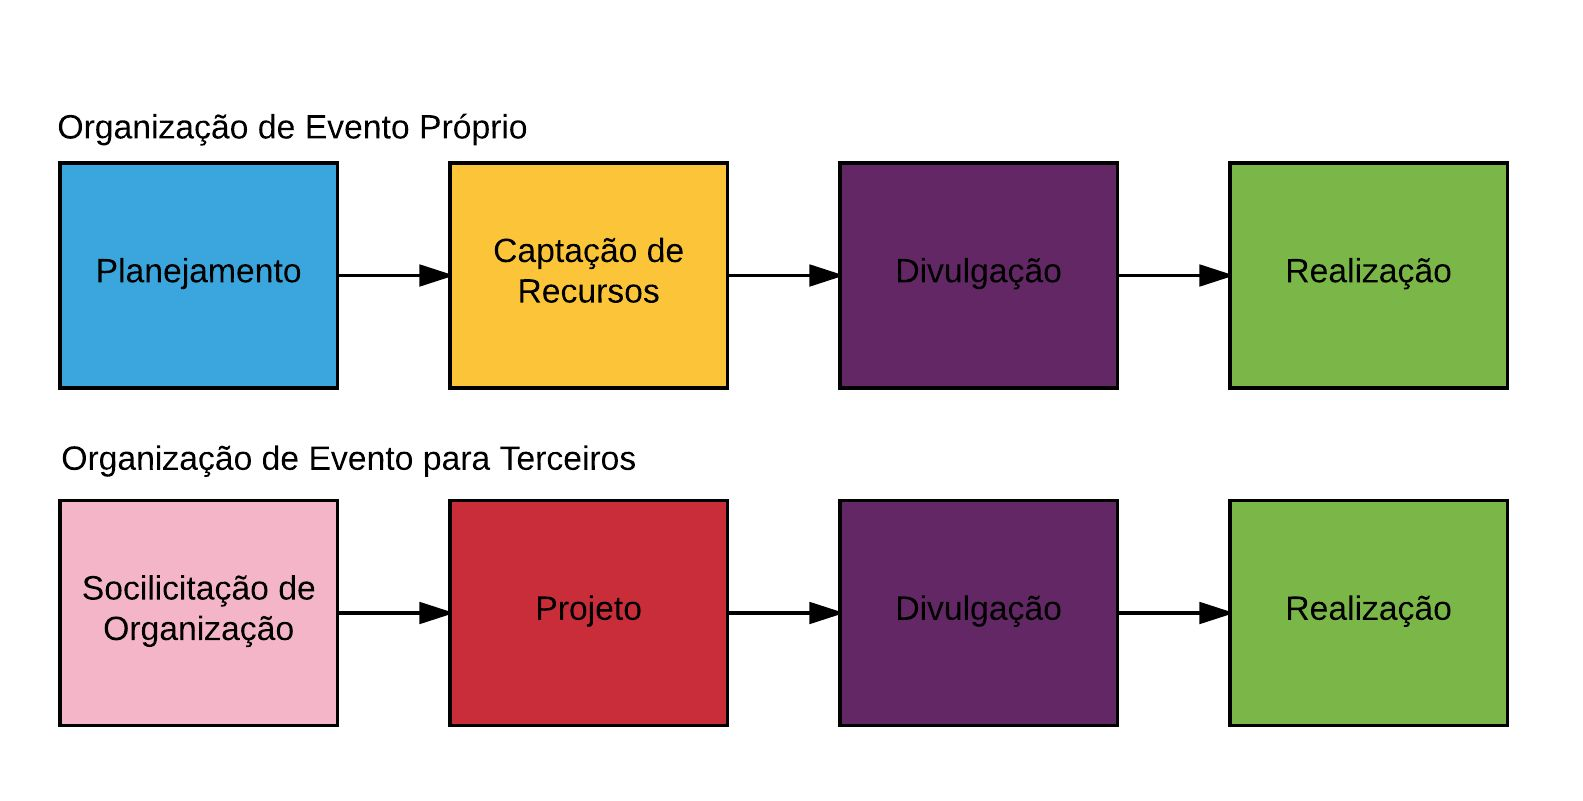
\includegraphics[scale=0.3]{img/img10.png}
    \caption{Processos Operacionais}
\end{figure}

Em um evento próprio, o conselho de planejamento formado pelas três diretorias, se reunirá e definirá as datas, fazendo assim um calendário anual com todos os eventos organizados pela empresa. O planejamento de cada evento deve conter todas as informações necessárias para sua organização - presencial ou não, número de participantes, premiação e outros. Na fase de captação de recursos, o departamento de marketing deverá propor ações de venda, merchandising, publicidade e propaganda, bem como a busca de patrocínio através de oferta de divulgação e/ou espaço para venda de produtos durante o evento, assim como da oferta dos dados, já tratados, conscientemente fornecidos pelos espectadores. Durante a captação de recursos, é importante alcançar o valor saudável definido pelo departamento financeiro. Na divulgação, serão realizadas propagandas nas principais redes sociais e comunidades gamers. A fase final de realização será responsabilidade da Diretoria Operacional, que deverá reunir a equipe pessoal necessária para a execução, preparar a infraestrutura e cuidar de qualquer imprevisto.

Em um evento organizado para terceiros, o comitê de planejamento oferecerá um projeto descritivo para o contratante, informando os custos e necessidades para a realização de um evento com o padrão solicitado. A divulgação e a realização serão executadas seguindo o mesmo modelo de organização própria.

\subsection{Necessidade inicial de colaboradores}
Estima-se que, de início, serão necessários os seguintes colaboradores desempenhando as seguintes funções:

\textbf{Diretor(a) de Finanças (CFO)} - Esse papel será assumido por um dos sócios. Suas responsabilidades serão: Administração dos riscos financeiros e planejamento financeiro da organização

\textbf{Diretor(a) de Marketing (CMO)} -  Esse papel será assumido por um dos sócios. Suas responsabilidades serão: Coordenar serviços de marketing na empresa,  propor ações de venda interna e externa, merchandising e programas de publicidade e propaganda. Analisar propostas de mídia e editoração de publicações internas e externas, visando promover o consumo de produtos e/ou utilização dos serviços oferecidos pela empresa.

\textbf{Diretor(a) de Operações (COO)} - Esse papel será assumido por um dos sócios. Suas responsabilidades são complexas: deve gerenciar o dia-a-dia das operações da empresa, bem como toda a operação dos eventos, que vai desde a organização até a execução

\textbf{Analista de Design} - Esse papel pode ser assumido por um colaborador contratado através de regime MEI (Microempreendedor Individual) ou ser terceirizado. Suas responsabilidades serão: conceber e confeccionar as mídias de divulgação da organização, de seus eventos e dos produtos a serem comercializados (camisas, canecas e outros)

\textbf{Narradores} - Será necessário, de início, um narrador para cada um dos jogos atendidos pela organização (5). Esse papel pode ser assumido por um colaborador contratado através de regime MEI (Microempreendedor Individual). Suas responsabilidades serão: Descrever oralmente as situações que ocorrem durante os jogos de forma dinâmica e descritiva.

\textbf{Comentaristas} - Será necessário, de início, um comentarista para cada um dos jogos atendidos pela organização (5). Esse papel pode ser assumido por um colaborador contratado através de regime MEI (Microempreendedor Individual). Suas responsabilidades serão: Analisar jogadas, escolhas e estratégias adotadas pelos times/jogadores durante os jogos, servirá de suporte ao narrador para transformar a transmissão em algo mais dinâmico.

\textbf{Observador(a)} -  Esse papel pode ser assumido por um colaborador contratado através de regime MEI (Microempreendedor Individual). Sua responsabilidade será guiar a câmera em alguns jogos (CS GO e Overwatch).

\textbf{Assessoria Contábil e Jurídica} - Esse papel pode ser assumido por uma empresa (ou indivíduo) terceirizada. Sua responsabilidade será assessorar a Diretoria da eVarsity com questões de caráter jurídico e financeiro.

\newpage
\section{Plano Financeiro}
\subsection{Investimentos Iniciais}
Os Investimentos Iniciais da eVarsity consistem na aquisição dos meios básicos para a realização dos Campeonatos Presenciais. Os meios básicos se dividem entre Computadores, Equipamentos de Rede e estrutura física. Outros gastos gerais, como infraestrutura local, iluminação, aparelhagem de som e servidores para realização de Campeonatos Online não seriam perenes. Segue relação do quantitativo de cada área de investimento:
\begin{table}[ht]
	\rowcolors{1}{}{}
	\centering
	\begin{tabular}{p{3.5cm}p{4.3cm}p{2cm}p{2cm}p{2.5cm}}
		\hline
		\cellcolor{gray}Descrição&\cellcolor{gray}Especificação&\cellcolor{gray}Quantidade&\cellcolor{gray}Valor Unitário&\cellcolor{gray}Total \\
		\hline
		Computadores&AMD FX-8320E 8GB HD 1TB VGA R7-360&12&R\$2.599,90&R\$31.198,80\\
		Servidor&HP ISS ML110 Gen9&1&R\$2.699,90&R\$2.699,90\\
		Switch&HP 1410-16 16-Portas&12&R\$330,00&R\$330,00\\
		Cabos de Redes&Tipos Variados&-/-&R\$300,00&R\$300,00\\
		Mesa Competição&5m x 1m&2&R\$750,00&R\$1.500,00\\
		Mesa Servidor&1.5m x 1m&1&R\$300,00&R\$300,00\\
		Projetor&Epson Powerlite W28+&1&R\$2.499,90&R\$2.499,90\\
		Tela de Projeção&TT07 com Tripé&1&R\$697,00&R\$697,00\\
		Abafadores de Ruído&3M Peltor&10&R\$32,00&R\$320,00\\
		Miscelânea&Adaptadores de Tomada, filtros de linha, extensões, etc&-/-&R\$1.000,00&R\$1.000,00\\
		\hline
		&&&\textbf{Total}&\textbf{R\$40.548,60}\\
		\hline
	\end{tabular}
\end{table}
\subsection{Capital de Giro}
O Capital de Giro necessário para a manutenção das atividades da eVarsity consiste nos gastos necessários para a manutenção dos equipamentos, para a operacionalização inicial de cada novo evento (lastro para pagar por serviços de impressão de material de divulgação e gastos operacionais com transporte dos Computadores e Materiais de Rede) e pelo pagamento das despesas operacionais a cada um dos trabalhadores da empresa que tomaram parte no último evento - tendo em vista o caráter inconstante dos ganhos da eVarsity, os empregados recebem pagamentos diretos em cada evento ao invés de receberem salários.

O valor do capital de giro seria estimado, então, em torno de 10\% do valor dos equipamentos (R\$4.054,86), adicionados a um capital base de R\$4.000,00 para iniciar novos eventos e a 20\% do lucro líquido gerado durante o último evento (estimado em R\$10.000,00). O valor do Capital de Giro da eVarsity, portanto, é estimado em R\$10.054,86.
\subsection{Investimentos Pré-Operacionais}
Considerando que todos os preparativos pré-operacionais (criação de identidade visual, concepção de divulgação, entre outros) serão exercidos por funcionários do próprio corpo fundador da eVarsity, não existe custo pré-operacional para a operação da empresa.
\subsection{Investimento Total}
O Investimento Total inicial, então, comporia a importância de R\$50,603,46.
\subsection{Estimativa de faturamento}
A característica dupla da prestação dos serviços da eVarsity torna a estimativa do faturamento da empresa um tanto quanto complexa. O espectador/jogador dos campeonatos organizados, embora também cliente potencial da empresa, se configura no principal mecanismo de barganha em relação aos principais clientes da empresa: as empresas patrocinadoras.

A estimativa de faturamento, portanto, deve conter a expectativa de patrocínio a ser recebido - o que varia com a quantidade de espectadores que os eventos atraem -, a possibilidade de venda de produtos secundários durante os eventos (camisas, canecas, etc.) - que também varia de acordo com a quantidade de espectadores - e a possível prestação de serviços/consultoria para outras organizações que desejem fazer eventos desse tipo.

Devem ser divididos os possíveis clientes, então, em 3 tipos: espectadores, patrocinadores e contratantes. Segue análise separada para cada um deles.
\subsubsection{Espectadores}

Para estimar o faturamento direto com os espectadores, é preciso, primeiramente, definir os tipos de receita que podem gerar:

1. Compra de merchandising dos eventos

2. Subscriptions e doações via Twitch

3. Ganho indireto com consumo de mídia em sites como YouTube.

Para estimar o faturamento possível em cada modalidade, deve-se primeiro estimar o mercado consumidor para cada modalidade.

\subsubsection{Merchandising}

A venda de merchandising, a curto prazo, será realizada dentro dos próprios eventos. Portanto, deve-se estimar a quantidade de possíveis espectadores presenciais para cada evento

Considerando que os eventos serão realizados, com certeza, no mínimo dentro da UFRJ, dentre todas as Universidades do estado do Rio de Janeiro, o grupo mínimo de universitários a ser afetado seria de 67.329 indivíduos (UFRJ, 2013). Considerando a estimativa pessimista de que aproximadamente 35\% dos alunos apresentam algum tipo de interesse em jogos eletrônicos, existe um mercado potencial de 23.565 pessoas. Considerando uma taxa de interesse de 10\%, e que os produtos só seriam atualizados uma vez por ano, podemos dizer que 2.356 pessoas/ano poderiam comprar merchandising apenas na UFRJ. Considerando um valor médio de R\$20,00 por compra - preço mínimo de venda de uma camisa - haveria um faturamento potencial de R\$47.120,00 por ano.

Quando expandindo os eventos para algumas das outras grandes universidades do Estado do Rio de Janeiro (UNIRIO - 11.141 alunos em 2014 - UFF - 51.422 alunos em 2013 - UERJ - 28.624 alunos em 2014 - PUC-Rio - 17.900 alunos em 2015) e mantendo-se a estimativa de 35\% de espectadores nos eventos e em 10\% a taxa de interesse nos produtos, o possível mercado consumidor se expande para 61.745 pessoas, e o faturamento potencial para R\$123.490,00. Considerando-se que nem todos os interessados efetivamente comprarão produtos repetidamente todos os anos, estimamos a média de receita por cliente em R\$5,00.

\subsubsection{Plataformas de Streaming}

A receita direta a ser obtida com os espectadores via plataformas de streaming condiz à inscrição direta mensal ao canal de streaming e a doações livres a serem operacionalizadas via PayPal. Cada inscrição rende U\$2,50 por mês, e as doações são livres. Considerando o meio de exposição, é possível afirmar que não apenas universitários podem compor o mercado consumidor, sendo impossível estimar a profundidade do mesmo. Convertendo o valor para reais na conversão direta de 19/11/2016, o consumo por consumidor, considerando ausência de doações e apenas meio ano de inscrição, gira em torno de R\$50,76/ano. Considerando-se uma média ainda mais baixa, com apenas um mês de inscrição em média, cada espectador gerará R\$8,50/ano.

\subsubsection{YouTube e Similares}
O mecanismo de monetização do YouTube consiste em um sistema chamado CPM, que remunera o produtor de conteúdo de acordo com 1.000 exibições de vídeo com propagandas de terceiros adicionadas. Segundo artigo do NYT de fevereiro de 2014\footnote{\url{http://www.nytimes.com/2014/02/02/business/chasing-their-star-on-youtube.html?_r=1}}, o CMP médio girava em torno de U\$7,60. Considerando a taxa retirada pelo próprio YouTube, cada 1000 visualizações geraria U\$4,18, ou  R\$13,95. Considerando que cada usuário pode assistir quantos vídeos desejar, e assistir o mesmo vídeo mais de uma vez, é impossível calcular com precisão a contribuição individual de cada cliente. É possível dizer porém, que o valor se mostre ínfimo para o cálculo final do faturamento por cliente.

O faturamento direto por Espectador, então, seria de R\$13,50/ano.

A longo prazo, é possível a cobrança de um valor para que cada espectador ingresse nas arenas onde estarão sendo realizados os torneios, o que aumentará consideravelmente o faturamento deste tipo de cliente. A curto prazo, porém, o caráter estritamente amador e Universitário dos torneios inviabiliza este tipo de cobrança.

\subsubsection{Patrocinadores}
Como dito anteriormente, os espectadores não são apenas mercado consumidor. Por se tratar de eventos universitários, os campeonatos se apresentam como excelente oportunidade de divulgação para empresas de que busquem se fazer conhecidas no meio. Empresas que busquem oportunidades de contratação de universitários de todas as áreas, especialmente daqueles que apresentem afinidade perante a área de Tecnologia da Informação - afinal, os campeonatos são desenvolvidos em cima de esportes eletrônicos - encontrarão um espaço fértil para divulgação própria e para obtenção de mailing lists e de indicações. Pode-se dizer que os principais clientes da eVarsity são as grandes contratantes de Universitários, especialmente empresas de Tecnologias, na forma de patrocinadoras.

Estimar o faturamento por patrocinador depende da estimativa de quantos espectadores pode-se contar com por evento. Novamente, considerando apenas o número de alunos da UFRJ e os 35\% estimados de interesse possível nos eventos, existe um mercado potencial de 23.565 indivíduos capacitados, em Cursos de Nível Superior de Universidade reconhecida, a serem diretamente afetados pelas ações de marketing dos possíveis patrocinadores. Considerando-se as outras Universidades já citadas, esse número beira os 61.745 indivíduos capacitados.

Considerando-se o interesse já apresentado, é possível realizar um cálculo de que cada espectador hoje vale, em média, R\$18,00, com tendência de crescimento. Considerando-se o potencial de 61.745 espectadores/ano, calcula-se um potencial de arrecadação de R\$1.111.410,00. Considerando-se a realização de múltiplos eventos por ano e a possibilidade de diferentes organizações patrocinarem cada um dos eventos, é difícil oferecer uma estimativa do Faturamento por Cliente neste caso.
As experiências anteriores, porém, nos permitem estimar um valor médio na importância de R\$15.000,00/evento por patrocinador individual.

\subsubsection{Serviços e Consultoria Externa}
\label{servcons}
O terceiro grupo de clientes da eVarsity é composto por contratantes que busquem uma empresa para organizar e operacionalizar campeonatos de esportes eletrônicos, sem a necessidade de que sejam de caráter exclusivamente Universitário. Considerando-se os custos operacionais e de garantia de materiais, a eVarsity cobra como taxa básica 10\% do valor dos equipamentos a serem utilizados por dia de duração do campeonato, adicionados de uma taxa variável de acordo com a expectativa média de público do evento a ser realizado e à contratação dos funcionários da eVarsity que trabalharão no evento.

O faturamento por cliente, então, não poderia ser menor do que R\$6.000 para um evento de um dia (R\$4.000,00 representando os 10\% dos materiais iniciais da eVarsity, R\$2,00 por espectador - ou 1000R\$ para os 500 espectadores esperados por um evento pequeno - e R\$1.000/(dia de 8 horas) dos salários do Staff mais reduzido possível). Um evento de semana inteira para os mesmos 500 espectadores, então, geraria uma receita de R\$10.000. Segue tabela:
\begin{table}[ht]
	\rowcolors{1}{}{}
	\centering
	\begin{tabular}{p{3.5cm}p{3.5cm}p{3.5cm}p{3.5cm}}
		\hline
		\cellcolor{gray}Descrição&\cellcolor{gray}Valor Unitário&\cellcolor{gray}Adicional por Dia&\cellcolor{gray}Estimativa\\
		\hline
		Materiais para realização dos Jogos (PCs e Rede)&15\% do Valor total dos Produtos + 2\% por diária + Diária do Administrador de Redes&Diária de Aluguel dos Equipamentos e do Administrador de Redes&10 PCS: R\$5,500
		Montagem: R\$1.000
		Diária dos Equipamentos:: R\$700,00
		Diária do Adm de Redes: R\$1.000,00\\
		\hline
		Narradores e Analistas para as Partidas&Salário dos Narradores/Analistas&Integral&Diária: R\$750,00 por Pessoa\\
		\hline
	\end{tabular}
\end{table}
\begin{table}[h!]
	\rowcolors{1}{}{}
	\centering
	\begin{tabular}{p{3.5cm}p{3.5cm}p{3.5cm}p{3.5cm}}
	Observador para as Partidas&Salário&Integral&Diária do Observador: R\$500,00\\
	\hline
	Material para Transmissão Offline (Projetor, Tela, PCs de Streaming)&10\% do Valor total dos Produtos + 2\% por diária&Diária de Aluguel dos Equipamentos&Infra Mínima: R\$500,00
	Diária dos Equipamentos: R\$100,00\\
	\hline
	Material para Transmissão Online (Configuração de Rede, Setup e Operação de Stream)&10\% do Valor total dos Produtos + Diária do Responsável pela Stream&Apenas Diária&Materiais: R\$500,00
	Diária do Responsável pela Stream: R\$1.000,00\\
	\hline
	Consultoria e Operação de Áudio para Casting Offline&10\% do Valor dos Produtos Utilizados + Montagem + Diária do Engenheiro de Áudio&Diária&Estudo e Montagem: R\$1000,00
	Materiais: R\$30,00
	Diária do Eng. de Áudio: R\$1.000,00\\
	\hline
	Consultoria para pós-produção ao vivo da Transmissão&Valor das Peças Produzidas + Adicional à Diária do Responsável pela Stream&Diária&Materiais Gráficos: R\$80,00 por Peça
	Adicional à Diária do Responsável da Stream: R\$500,00\\
	\hline
	Admins Para as Partidas&Diária dos Admins&Integral&Diária: R\$500,00 para cada duas pessoas.\\
	\hline
	Embelezamento da Arena e Iluminação da Mesa de Narração&80\% do Valor do Aluguel dos Produtos Utilizados + Salário da Montagem&Nenhum&Materiais: R\$6.000,00
	Montagem: R\$1.000,00\\
	\hline
	Múltiplas Linhas de Vídeo na Stream: Operação de Câmeras&80\% do Valor do Aluguel dos Produtos Utilizados + Montagem + Diária dos Operadores de Câmera + Diária do Diretor de Vídeo&Diárias&Materiais: R\$10.000,00
	Montagem: R\$1.000,00
	Diária Operadores de Câmera: R\$750,00 por Pessoa
	Diária do Diretor de Vídeo: R\$1.500,00\\
	\hline
\end{tabular}
\end{table}
\newpage
Um evento completo teria, então, custo fixo de ao contratante na casa dos R\$23.330,00 para materiais e na casa dos R\$4.000,00 para montagem, além de um custo variável com uma diária mínima na casa dos R\$7.500,00 considerando-se o mínimo possível de 7 pessoas e um evento de apenas um dia, num total de R\$34.380,00.

Caso o Cliente já possua os materiais necessários à realização do evento, serão cobrados apenas os valores dos salários dos funcionários, além do valor de montagem das estruturas, de um valor a ser combinado de acordo com o número de espectadores do evento e de divulgação abrangente da eVarsity como sua firma de produção.
Considerando-se que a maioria dos eventos, a curto prazo, não envolveria todos os módulos e se estenderia entre 1 e 3 dias, estimamos o faturamento médio por cliente na casa dos R\$12.000,00.
\subsection{Estimativa do custo do serviço}
Como a atividade da eVarsity se baseia na produção de eventos e na venda de espaço de patrocínio, é difícil estimar um valor fixo para seus custos operacionais. Para tentar aproximar um valor para este quesito, dividem-se os custos entre Custos de Operação Online - quando o Campeonato só é realizado via Internet - e Custos de Operação \textit{in Loco} - quando o Campeonato é presencial.

\textbf{Custos de Operação Online:}

Aluguel de Servidores Para Hospedagem dos Jogos: R\$85,00/mês/Servidor

Administradores do Torneio: R\$200,00/mês/pessoa

Produção de Peças de Divulgação Online: R\$80,00/peça

Produção de Vídeos de Divulgação: R\$300,00/vídeo

Premiação dos Vencedores: Variável entre não-existente e R\$1.000,00


Custo médio por Torneio Online: R\$1.000

\textbf{Custos de Operação \textit{In Loco:}}

Transporte dos materiais até o local de realização do evento: Média de R\$800,00

Diárias dos Funcionários: Variável para cada tipo de Evento. Mínimo de R\$7.500,00 para um evento completo de um dia com o mínimo Staff possível, ou de R\$2.500,00 para o menor evento possível, também de um dia e também com mínimo Staff possível.

Custos com Aluguel de Equipamentos extras: Variáveis entre não-existentes e R\$16.000,00

Custos com Adaptação do Espaço: Variáveis entre não-existentes e R\$2.000,00

Custos com Aluguel do Espaço: Variáveis entre não-existentes e R\$10.000,00

Premiação dos Vencedores: Variável entre R\$600,00 e R\$1.500,00

Produção de Peças de Divulgação Online: R\$80,00/peça

Custo médio por Torneio In Loco: R\$6.000,00 para torneios externos (sem recebimento de Patrocínio) e R\$10.000,00 para torneios internos (com recebimento de Patrocínio).

\subsubsection{Estimativa de Custo de Comercialização}
Os principais custos de Comercialização da eVarsity serão as taxas cobradas sobre as transferências bancárias para recebimento das cotas dos patrocinadores e de eventuais taxações sobre a venda de merchandising, caso seja utilizada máquina de cartão para sua venda, e sobre o recebimento do valor de inscrições e doações online devido à taxa de operação de serviços como PayPal e PagSeguro. Estima-se essas taxas em uma média de 5\% do arrecadamento bruto das atividades distintas da eVarsity.

\subsubsection{Provisão para Devedores Duvidosos}
Considerando o caráter imediato das vendas de merchandising e do recebimento dos valores de inscrição e doação em mídias sociais, assim como a assinatura de contratos para o recebimento das cotas de patrocínio, fica a eVarsity imune ao risco de inadimplência, não sendo necessária, portanto, armazenagem de capital para PDD.

\subsection{Custos com Depreciação}
Observando os itens adquiridos para a manutenção de servidores e produção de eventos, vemos que diversos itens sofrem uma depreciação que deve ser contabilizada. Sendo assim foram contabilizados custos de 20\% a.a. para os computadores, cabos de rede, switch e servidor.

\begin{table}[ht]
	\rowcolors{1}{}{}
	\centering
	\begin{tabular}{p{3.5cm}p{2cm}p{3cm}p{3.5cm}p{2.5cm}}
		\hline
		\cellcolor{gray}Equipamento&\cellcolor{gray}Referência NCM&\cellcolor{gray}Prazo de vida útil (anos)&\cellcolor{gray}Taxa de Depreciação Anual (\%)&\cellcolor{gray}Depreciação \\
		\hline
		Computadores&8471&5&20&R\$6.239,60\\
		Cabos de Rede&8471&5&20&R\$60,00\\
		Switch&8471&5&20&R\$66,00\\
		Servidor&8471&5&20&R\$539,98\\
		Mesa Competição&8471&10&10&R\$150,00\\
		Mesa Servidor&9403&10&10&R\$30,00\\
		Projetor&8525&5&20&R\$499,80\\
		Tela de Projeção&9010&10&10&R\$ 69,70\\
		\hline
		&&&\textbf{Total}&\textbf{R\$7.655,08}\\
		\hline
	\end{tabular}
\end{table}
\subsection{Custos Operacionais}
Considerando a característica variável das operações da eVarsity, os custos operacionais foram separados em três categorias: manutenção das Plataformas Online, Custo de Operação de Torneios Online e Custo de Operação de Torneios In Loco. Cada uma dessas categorias, por sua vez, foi dividida em dois tipos de análise de despesa: custos mensais, perenes, e custos esperados para a realização de eventos, momentâneos. Os custos para realização de eventos será tratado como gasto mensal médio, através de cálculo que considera a quantidade média de eventos a serem realizados por ano (dois In  Loco e 8 online) e o valor médio de custo de cada um deles (R\$8.000,00 para In Loco e R\$1.000,00 para online.

\begin{table}[ht]
	\rowcolors{1}{}{}
	\centering
	\begin{tabular}{p{6cm}p{7cm}p{2cm}}
		\hline
		\cellcolor{gray}Manutenção das plataformas online&\cellcolor{gray}Custo Mensal&\cellcolor{gray}Custo por evento\\
		\hline
		Hospedagem do Website&Administrador de Página: R\$50,00&Nulo\\
		Atualização de Página no Facebook e no Twitter&Aluguel de Servidor: R\$40,00
		Manutenção: R\$50,00&Nulo\\
		Youtube&Editor e Produtor de Vídeos: R\$80,00&Nulo\\
		Concepção de Peças de Divulgação para todas as Plataformas&Designer: R\$80,00
		Média de 1 Peça/mês&Nulo\\
		\hline
	\end{tabular}
\end{table}

\begin{table}[ht]
	\rowcolors{1}{}{}
	\centering
	\begin{tabular}{p{6cm}p{7cm}p{2cm}}
		\hline
		\cellcolor{gray}Custos de realização de eventos&\cellcolor{gray}Custo Mensal&\cellcolor{gray}Custo por evento\\
		\hline
		Eventos Online&R\$667,00&R\$1.000,00 \\
		Eventos In Loco&R\$1.334,00&R\$8.000,00 \\
		\hline
	\end{tabular}
\end{table}

\begin{table}[ht]
	\rowcolors{1}{}{}
	\centering
	\begin{tabular}{p{6cm}p{7cm}p{2cm}}
		\hline
		\cellcolor{gray}Custos Variados&\cellcolor{gray}Custo Mensal&\cellcolor{gray}Custo por evento\\
		\hline
		Aluguel do Espaço para Armazenagem dos PCs&R\$300,00&Nulo  \\
		Pagamento de Salários para o Conselho Gestor& 40\% do Lucro Líquido da Empresa&Nulo \\
		\hline
	\end{tabular}
\end{table}
\newpage
Gasto Mensal Total Estimado: R\$2.601,00 + 5\% do Lucro Líquido

Gasto Total Anual Estimado: R\$31.212,00 + 5\% do Lucro Líquido

\subsection{DRE}
A realização do DRE para a eVarsity se mostra bastante complexo na medida em que, novamente, esbarra na multiplicidade de seus clientes. Para simplificar a realização do Demonstrativo de Resultado de Exercício, utilizaremos uma progressão em relação ao mercado Universitário de espectadores interessados.

Consideraremos como número total de clientes o número de alunos de Universidades do Estado do Rio de Janeiro. Considerando-se as grandes Universidades já previamente citadas, teremos um número de 176,415 alunos. Adicionando-se a esses números também Universidades como UVA (24.500 alunos), UNESA (108.468 alunos), UNICARIOCA (6.000 alunos) FGV, IBMEC e FACHA o número pode chegar a mais de 300.000 indivíduos. Mesmo considerando-se a estimativa já utilizada de apenas 35\% desses indivíduos poderem ser direta ou indiretamente afetados pela eVarsity, o número estimado de potenciais clientes ainda se mantém em mais de 100.000.

O percentual desses consumidores estabelecido como meta de demanda efetiva é de 10\% de todos os consumidores potenciais até o ano 4. Partindo da quantidade já afetada (1.500 pessoas, ou 1,5\% do total), é possível prever um crescimento linear de 2,85\% até os 3 anos iniciais e um crescimento incremental que obedece à regra (30 - 2t)\%, onde t é ano, considerando o 4 ano como ano inicial, até o décimo ano.

\begin{table}[ht]
	\rowcolors{1}{}{}
	\centering
	\begin{tabular}{p{1cm}p{4.5cm}p{4.2cm}p{4cm}}
		\hline
		\cellcolor{gray}Ano&\cellcolor{gray}Número de Espectadores&\cellcolor{gray}Crescimento Anual (\%)&\cellcolor{gray}\% dos clientes totais\\
		\hline
		1&1.500&-&1.5\\
		2&4.350&190&4.35\\
		3&7.200&65.5&7.2\\
		4&10.000&39.5&10.05\\
		5&13.000&30&13\\
		6&16.640&28&16.6\\
		7&20.967&26&20.97\\
		8&25.998&24&25.99\\
		9&31.718&22&31.72\\
		10&38.062&20&38.6\\
		\hline
	\end{tabular}
\end{table}

A partir desses dados, é possível aplicar os valores apresentados no item 4.5 para duas das três áreas: Faturamento Direto com Espectadores e Faturamento com Patrocinadores. Considerando-se o Faturamento médio por cliente diretamente dos espectadores como R\$13,50 e dos Patrocinadores como R\$18,00 por indivíduo afetado, é possível calcular a receita potencial anual da eVarsity.

\begin{table}[ht]
	\rowcolors{1}{}{}
	\centering
	\begin{tabular}{p{1cm}p{3cm}p{3.5cm}p{3.5cm}p{3cm}}
		\hline
		\cellcolor{gray}Ano&\cellcolor{gray}Número de Espectadores&\cellcolor{gray}Receita Direta com Espectadores (R\$)&\cellcolor{gray}Receita via Patrocinadores(R\$)&\cellcolor{gray}Total (R\$)\\
		\hline
		1&1.500&20.250,00&27.000,00&47.250,00\\
		2&4.350&58.725,00&78.300,00&137.025,00\\
		3&7.200&97.200,00&129.600,00&226.800,00\\
		4&10.000&135.000,00&180.000,00&315.000,00\\
		5&13.000&175.500,00&234.000,00&409.500,00\\
		6&16.640&224.640,00&299.520,00&524.160,00\\
		7&20.967&283.054,00&377.406,00&660.460,00\\
		8&25.998&350.973,00&467.964,00&818.937,00\\
		9&31.718&428.193,00&570.924,00&999.117,00\\
		10&38.062&513.837,00&685.116,00&1.198.953,00\\
		\hline
	\end{tabular}
\end{table}

Vale lembrar que essa tabela não inclui o potencial oferecimento de Consultoria/Prestação de Serviços, uma das categorias da atuação da eVarsity, pela ausência de capacidade de estimativa em relação ao número de potenciais clientes. Apenas para fins de estimativa conservadora, serão adicionados R\$10.000,00 +R\$3.000,00/por ano a partir do Ano 2 para efeito de contabilidade.

Considera-se também que no ano 4 e no ano 8 adiciona-se 1 evento presencial e 4 online anuais a serem realizados, o que aumenta os custos operacionais. Entre os anos 1 e 3, o CSP é de R\$24012,00/ano; entre os anos 4 e 7 o CSP é de R\$36012,00/ano e, entre os anos 8 e 10 o CSP é de R\$48012,00/ano.

Considera-se também que, juntamente ao crescimento do número de eventos realizados, dobra o custo das Despesas Operacionais anuais. Portanto, a partir do ano 4 as DO passam a somar a importância de 14400 e, a partir do ano 8, a somar a importância de 28800.

Com esses dados, portanto, é possível finalmente confeccionar o DRE.

\begin{landscape}
	\begin{table}[ht]
		\rowcolors{1}{}{}
		\centering
		\begin{tabular}{p{5cm}p{1.5cm}p{1.5cm}p{1.5cm}p{1.5cm}p{1.5cm}p{1.5cm}p{1.5cm}p{1.5cm}p{1.5cm}p{1.5cm}}
			\hline
			\cellcolor{gray}Ano & \cellcolor{gray}1 & \cellcolor{gray}2 & \cellcolor{gray}3 & \cellcolor{gray}4 & \cellcolor{gray}5 & \cellcolor{gray}6 & \cellcolor{gray}7 & \cellcolor{gray}8 &\cellcolor{gray} 9 & \cellcolor{gray}10 \\ \hline
			Clientes & 1500 & 4350 & 7200 & 10000 & 13000 & 16640 & 20967 & 25998 & 31718 & 38062 \\ \hline
			Crescimento (\%) & - & 190 & 65 & 39 & 30 & 28 & 26 & 24 & 22 & 20 \\ \hline
			Receita Bruta & 57250 & 150025 & 242800 & 334000 & 430500 & 549160 & 688460 & 849937 & 1033117 & 1235953 \\ \hline
			Impostos & 9160 & 24004 & 38848 & 53440 & 68880 & 87866 & 110154 & 135990 & 165299 & 197753 \\ \hline
			Receita Líquida & 48090 & 126021 & 203952 & 280560 & 361620 & 461294 & 578306 & 713947 & 867818 & 1038200 \\ \hline
			CSP & 24012 & 24012 & 24012 & 36012 & 36012 & 36012 & 36012 & 48012 & 48012 & 48012 \\ \hline
			Depreciação & 7655 & 7655 & 7655 & 7655 & 7655 & 7655 & 7655 & 7655 & 7655 & 7655 \\ \hline
			Lucro Bruto & 16423 & 94354 & 172285 & 236893 & 317953 & 417627 & 534639 & 658280 & 812151 & 982533 \\ \hline
			Custo de Comercialização & 2862 & 7501 & 12140 & 16700 & 21525 & 27458 & 34423 & 42497 & 51656 & 61798 \\ \hline
			Despesas Operacionais & 7200 & 7200 & 7200 & 14400 & 14400 & 14400 & 14400 & 28800 & 28800 & 28800 \\ \hline
			Lucro Líquido & 6361 & 79653 & 152945 & 205793 & 282028 & 375769 & 485816 & 586983 & 731695 & 892001 \\ \hline
			Margem Líquida (\%) & 11 & 53 & 63 & 62 & 66 & 68 & 70 & 69 & 71 & 72 \\ \hline
			Lucro Final (após desconto de salários) & 3817 & 47792 & 91767 & 123476 & 169217 & 225461 & 291489 & 352190 & 439017 & 535201 \\ \hline
			Lucro Acumulado & 3817 & 51609 & 143366 & 266842 & 436059 & 661520 & 953009 & 1305199 & 1744216 & 2279417 \\ \hline
		\end{tabular}
	\end{table}
\newpage
\subsection{O Fluxo de Caixa}
Com o DRE completo é possível elaborar uma projeção do fluxo de caixa anual da eVarsity. Para essa elaboração, consideramos que o custo de depreciação é reinvestido no exercício seguinte e que os investimentos iniciais serão realizados através de capital próprio.

	\begin{table}[ht]
		\rowcolors{1}{}{}

		\begin{tabular}{p{5cm}p{1.2cm}p{1.2cm}p{1.2cm}p{1.2cm}p{1.2cm}p{1.2cm}p{1.2cm}p{1.2cm}p{1.2cm}p{1.2cm}p{1.2cm}}
		\hline
			\cellcolor{gray}Ano & \cellcolor{gray}0 & \cellcolor{gray}1 & \cellcolor{gray}2 & \cellcolor{gray}3 & \cellcolor{gray}4 & \cellcolor{gray}5 & \cellcolor{gray}6 & \cellcolor{gray}7 & \cellcolor{gray}8 &\cellcolor{gray} 9 & \cellcolor{gray}10 \\ \hline
	Lucro Final & 0 & 3817 & 47792 & 91767 & 123476 & 169217 & 225461 & 291489 & 352190 & 439017 & 535201 \\ \hline
	Depreciação & 0 & 7655 & 7655 & 7655 & 7655 & 7655 & 7655 & 7655 & 7655 & 7655 & 7655 \\ \hline
	Capex & 0 & 0 & 7655 & 7655 & 7655 & 7655 & 7655 & 7655 & 7655 & 7655 & 7655 \\ \hline
	Capital de Giro & 10058 & 0 & 0 & 0 & 0 & 0 & 0 & 0 & 0 & 0 & 0 \\ \hline
	Investimentos & 50604 & 0 & 0 & 0 & 0 & 0 & 0 & 0 & 0 & 0 & 0 \\ \hline
	Financiamen. & 0 & 0 & 0 & 0 & 0 & 0 & 0 & 0 & 0 & 0 & 0 \\ \hline
	Fluxo de Caixa Livre & -40546 & 21530 & 69322 & 161089 & 284565 & 453782 & 679243 & 970732 & 1322922 & 1761939 & 2297140 \\ \hline
		\end{tabular}
	\end{table}

\end{landscape}

\subsection{Indicadores de Viabilidade}
Utilizando os dados obtidos de fluxo de caixa, podemos analisar diferentes indicadores de viabilidade para a empresa. Começaremos com o Valor Presente Líquido com uma Taxa Mínima de Atratividade fixada em 10\% ao ano.

	\begin{table}[ht]
		\rowcolors{1}{}{}
				\centering
		\begin{tabular}{p{3cm}p{5cm}}
	\hline
	\cellcolor{gray}Anos &\cellcolor{gray}VPL (em Mil reais) \\ \hline
	0 & -40.6 \\ \hline
	1 & 21.53 \\ \hline
	2 & 63.02 \\ \hline
	3 & 133.13 \\ \hline
	4 & 213.8 \\ \hline
	5 & 309.94 \\ \hline
	6 & 421.76 \\ \hline
	7 & 548 \\ \hline
	8 & 678.87 \\ \hline
	9 & 821.96 \\ \hline
	10 & 974.21 \\ \hline
	Total & 4145.62 \\ \hline
		\end{tabular}
	\end{table}

Nesse prazo de 10 anos o Retorno sobre o Investimento (ROI) chega ao surpreendente valor de 10223\%. A Taxa Interna de Retorno (TIR), calculada através do Fluxo de Caixa, aproxima-se à 566\% a.a.. O tempo de payback descontado, considerando-se uma taxa de juros fixada a 11,5\% a.a., é estimada em 1 ano e 7 meses, o que pode ser considerado bastante curto.

Estes indicadores parecem confirmar excelentes possibilidade de ganho e um curto tempo de retorno integral dos investimentos iniciais. Os valores do TIR e do ROI, se confirmadas reais, representariam um investimento com retorno altíssimo para um investimento ínfimo de menos de meia centena de milhar de reais.
\subsection{Cenário Alternativo}
Como os indicadores de retorno sobre o investimento previamente calculados se mostraram, talvez, excessivamente promissores, realiza-se aqui a concepção de um cenário extremamente pessimista, a fim de balizar por baixo os riscos do empreendimento. Nesse cenário, será reduzido o alcance da eVarsity no mercado consumidor através das seguintes medidas:

A porcentagem de impacto da eVarsity na comunidade universitária será reduzida de 35\% do corpo docente para 15\% do corpo docente (45.000 pessoas).

O prazo para que as operações da eVarsity atinjam os mesmos 10\% do potencial mercado consumidor será de 8 anos, ao invés de 4.

Após levar esses dados em consideração, existe um outro DRE:

\begin{table}[ht]
	\rowcolors{1}{}{}
	\centering
	\begin{tabular}{p{1cm}p{4.5cm}p{4.2cm}p{4cm}}
		\hline
		\cellcolor{gray}Ano&\cellcolor{gray}Número de Espectadores&\cellcolor{gray}Crescimento Anual (\%)&\cellcolor{gray}\% dos clientes totais\\
		\hline
	1 & 1500 & - & 3.34 \\
	2 & 1931 & 29 & 4.29 \\
	3 & 2358 & 22 & 5.24\\
	4 & 2786 & 18 & 6.19 \\
	5 & 3213 & 15 & 7.14 \\
	6 & 3641 & 13 & 8.09 \\
	7 & 4073 & 12 & 9.05 \\
	8 & 4500 & 11 & 10 \\
	9 & 4950 & 10 & 31.72 \\
	10 & 5445 & 10 & 38.06 \\ \hline
		\end{tabular}
	\end{table}

\begin{table}[ht]
	\rowcolors{1}{}{}
	\centering
	\begin{tabular}{p{1cm}p{3cm}p{3.5cm}p{3.5cm}p{3cm}}
		\hline
		\cellcolor{gray}Ano&\cellcolor{gray}Número de Espectadores&\cellcolor{gray}Receita Direta com Espectadores (R\$)&\cellcolor{gray}Receita via Patrocinadores(R\$)&\cellcolor{gray}Total (R\$)\\
		\hline
	1 & 1500 & 20520 & 27000 & 47520 \\
	2 & 1931 & 26069 & 34758 & 60827 \\
	3 & 2358 & 31833 & 42444 & 74277 \\
	4 & 2786 & 37611 & 50148 & 87759 \\
	5 & 3213 & 43376 & 57834 & 101210 \\
	6 & 3541 & 47804 & 63738 & 111542 \\
	7 & 4073 & 54985 & 73314 & 128299 \\
	8 & 4500 & 60750 & 81000 & 141750 \\
	9 & 4950 & 66825 & 89100 & 155925 \\
	10 & 5445 & 73508 & 98010 & 171528 \\ \hline
		\end{tabular}
	\end{table}

\newpage
Nesse caso, a solução para a dificuldade de estimativa do serviço de Consultoria/Prestação de Serviços consistirá no adicional de R\$10.000,00 +R\$1.000,00/por ano a partir do Ano 2 para efeito de contabilidade.

Nesse caso, também, considerando-se o pequeno aumento do mercado consumidor, não haverá incremento no número de campeonatos realizados e, portanto, o CSP se manterá estável em R\$24.012,00/ano.

Pelo mesmo motivo, não haverá aumento das Despesas Operacionais nos anos 4 e 8 do DRE.

\begin{landscape}
	\begin{table}[ht]
		\rowcolors{1}{}{}
		\centering
		\begin{tabular}{p{5cm}p{1.5cm}p{1.5cm}p{1.5cm}p{1.5cm}p{1.5cm}p{1.5cm}p{1.5cm}p{1.5cm}p{1.5cm}p{1.5cm}}
			\hline
			\cellcolor{gray}Ano & \cellcolor{gray}1 & \cellcolor{gray}2 & \cellcolor{gray}3 & \cellcolor{gray}4 & \cellcolor{gray}5 & \cellcolor{gray}6 & \cellcolor{gray}7 & \cellcolor{gray}8 &\cellcolor{gray} 9 & \cellcolor{gray}10 \\ \hline
	Clientes & 1500 & 1931 & 2358 & 2786 & 3213 & 3541 & 4073 & 4500 & 4950 & 5445 \\ \hline
	Crescimento & - & 29 & 22 & 18 & 15 & 13 & 12 & 11 & 10 & 10 \\ \hline
	Ano  & 1 & 2 & 3 & 4 & 5 & 6 & 7 & 8 & 9 & 10 \\ \hline
	Receita Bruta & 57520 & 71827 & 86277 & 100759 & 115210 & 126542 & 145299 & 159750 & 174925 & 191528 \\ \hline
	Impostos & 9203 & 11492 & 13804 & 16121 & 18434 & 20246 & 23248 & 25560 & 27988 & 30644 \\ \hline
	Receita Líquida & 48317 & 60335 & 72473 & 84638 & 96776 & 106296 & 122051 & 134190 & 146937 & 160884 \\ \hline
	CSP & 24012 & 24012 & 24012 & 24012 & 24012 & 24012 & 24012 & 24012 & 24012 & 24012 \\ \hline
	Depreciação & 7655 & 7655 & 7655 & 7655 & 7655 & 7655 & 7655 & 7655 & 7655 & 7655 \\ \hline
	Lucro Bruto & 16650 & 28668 & 40806 & 52971 & 65109 & 74629 & 90384 & 102523 & 115270 & 129217 \\ \hline
	Custo de Comercialização & 2876 & 3591 & 4314 & 5038 & 5760 & 6327 & 7265 & 7987 & 8746 & 9576 \\ \hline
	Despesas Operacionais & 7200 & 7200 & 7200 & 7200 & 7200 & 7200 & 7200 & 7200 & 7200 & 7200 \\ \hline
	Lucro Líquido & 6574 & 17877 & 29292 & 40733 & 52149 & 61102 & 75919 & 87336 & 99324 & 112441 \\ \hline
	Margem Líquida & 11 & 25 & 34 & 40 & 45 & 48 & 52 & 55 & 57 & 59 \\ \hline
	Lucro Final (após desconto de salários) & 3944 & 10726 & 17575 & 24440 & 31289 & 36661 & 45551 & 52402 & 59594 & 67465 \\ \hline
	Lucro Acumulado & 3944 & 14670 & 32245 & 56685 & 87974 & 124635 & 170186 & 222588 & 282182 & 349647 \\ \hline
		\end{tabular}
		\begin{tabular}{p{6.2cm}p{1.2cm}p{1.2cm}p{1.2cm}p{1.2cm}p{1.2cm}p{1.2cm}p{1.2cm}p{1.2cm}p{1.2cm}p{1.2cm}p{1.2cm}}
			\cellcolor{gray}Ano & \cellcolor{gray}0 & \cellcolor{gray}1 & \cellcolor{gray}2 & \cellcolor{gray}3 & \cellcolor{gray}4 & \cellcolor{gray}5 & \cellcolor{gray}6 & \cellcolor{gray}7 & \cellcolor{gray}8 &\cellcolor{gray} 9 & \cellcolor{gray}10 \\ \hline
			Lucro Final & 0 & 3944 & 10726 & 17575 & 24440 & 31289 & 36661 & 45551 & 52402 & 59594 & 67465 \\ \hline
			Depreciação & 0 & 7655 & 7655 & 7655 & 7655 & 7655 & 7655 & 7655 & 7655 & 7655 & 7655 \\ \hline
			Capex & 0 & 0 & 7655 & 7655 & 7655 & 7655 & 7655 & 7655 & 7655 & 7655 & 7655 \\ \hline
			Capital de Giro & 10058 & 0 & 0 & 0 & 0 & 0 & 0 & 0 & 0 & 0 & 0 \\ \hline
			Investimentos & 50604 & 0 & 0 & 0 & 0 & 0 & 0 & 0 & 0 & 0 & 0 \\ \hline
			Financiamen. & 0 & 0 & 0 & 0 & 0 & 0 & 0 & 0 & 0 & 0 & 0 \\ \hline
			Fluxo de Caixa Livre & -40546 & 21657 & 32383 & 49958 & 74398 & 105687 & 142348 & 187899 & 240301 & 299895 & 367360 \\ \hline
		\end{tabular}
	\end{table}


	\end{landscape}

A Análise VPL, então, segue abaixo.

	\begin{table}[ht]
		\rowcolors{1}{}{}
		\centering
		\begin{tabular}{p{3cm}p{5cm}}
			\hline
			\cellcolor{gray}Anos &\cellcolor{gray}VPL (em Mil reais) \\ \hline
	0 & -40.55 \\
	1 & 21.66 \\
	2 & 29.44 \\
	3 & 41.29 \\
	4 & 55.9 \\
	5 & 72.19 \\
	6 & 88.39 \\
	7 & 106.06 \\
	8 & 123.31 \\
	9 & 139.9 \\
	10 & 155.8 \\
	Total & 793.38 \\
		\end{tabular}
	\end{table}

O Retorno sobre o Investimento, neste caso, ronda os 1956\%. A Taxa Interna de Retorno, a partir deste novo Fluxo de Caixa, orbita os 91\% a.a.. O tempo de Payback neste novo cenário, considerando-se a mesma taxa fixa de juros anual, é de 3 anos e 5 meses.

Mesmo com uma redução considerável no Lucro Líquido, na ordem de 85\%, devido à redução de 86\% do Mercado Consumidor aplicada à nova estimativa de alcance da eVarsity, é possível considerar que a empresa ainda se mostra um investimento viável, porém de retorno menor e mais lento. A TIR de 91\%a.a., considerando-se o ínfimo investimento inicial, e o tempo mais lento, porém não tão grande, de recuperação dos investimentos, assim como a capacidade de operar no positivo já a partir do primeiro ano, mesmo com mercado reduzido, ainda fazem da eVarsity uma boa opção para investimento.

A conquista de um mercado consumidor mais extenso, porém, pode ser a diferença entre a empresa se constituir em um bom investimento ou em um investimento excelente. Mostram-se importantes ações de divulgação e cooptação extensivas para máximo retorno do investimento.
\newpage
\begin{landscape}
\section{Estrutura da Empresa}
\subsection{Estrutura Organizacional}
    \begin{figure}[!ht]
    	\centering
    	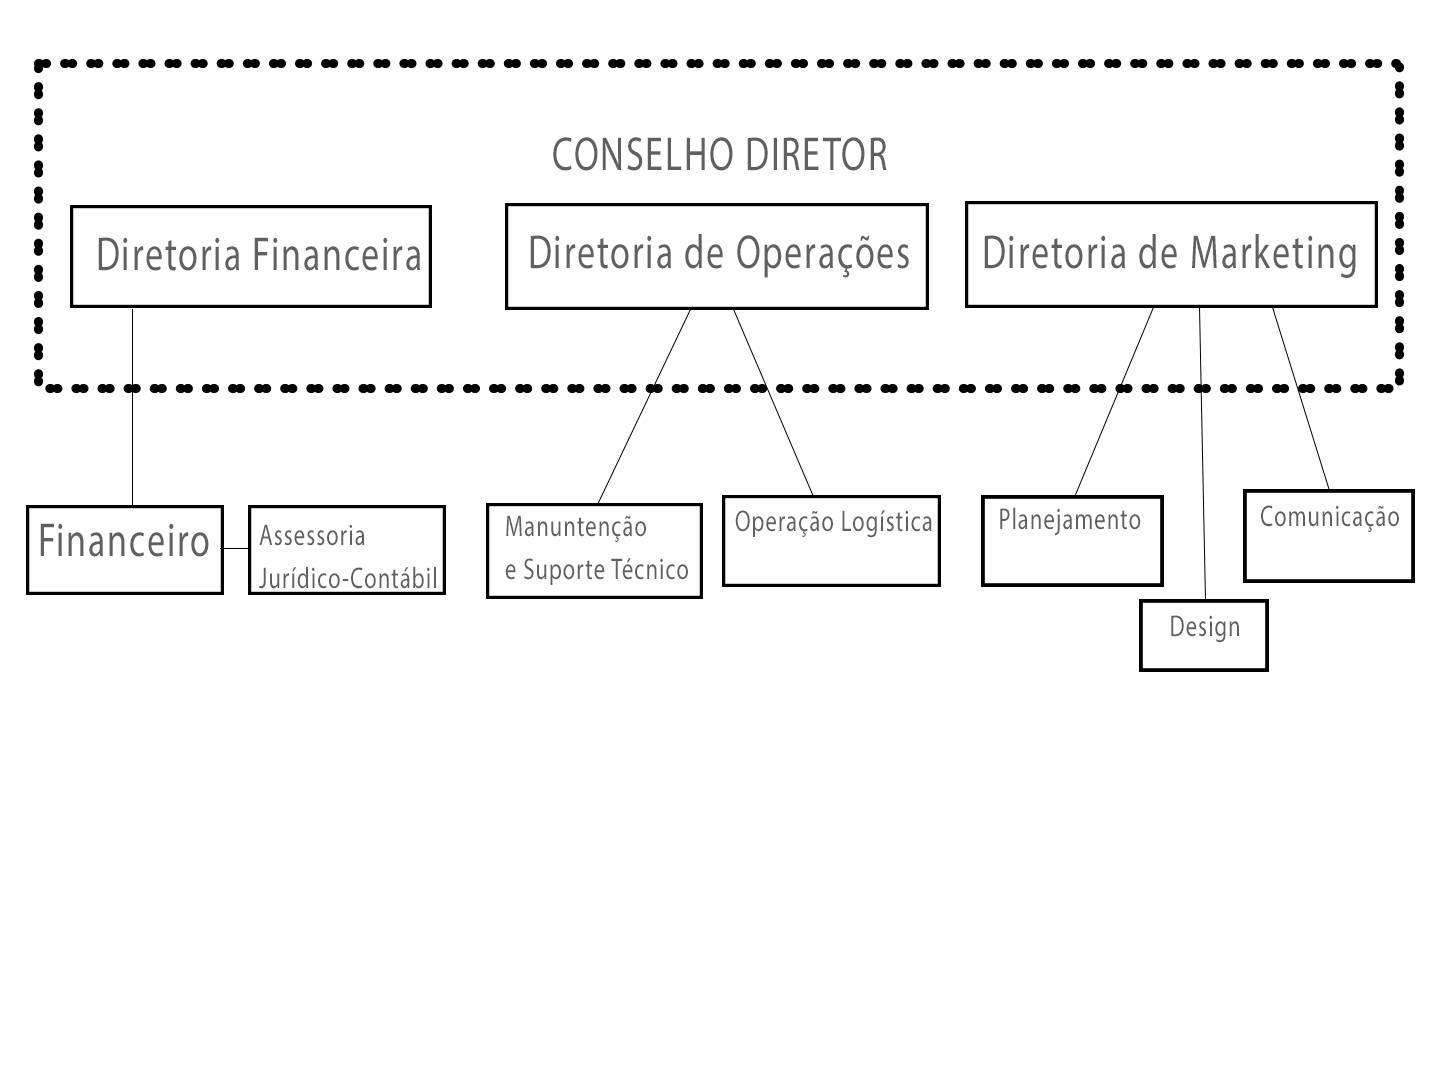
\includegraphics[width=25cm,height=12cm]{img/img09.jpg}
    	\caption{Organograma}
    \end{figure}
\end{landscape}

\textbf{Conselho diretor} - Conselho deliberativo onde cada diretoria possui um voto, independente do n\'{u}mero de diretores, para definir os rumos da organiza\c{c}\~{a}o.

\textbf{Diretoria Financeira} - Diretoria respons\'{a}vel pela Administração dos riscos financeiros e planejamento financeiro da organização

\textbf{Departamento Financeiro} - Departamento auxiliar as atividades da diretoria financeira.

\textbf{Acessoria Jur\'{i}dico-Cont\'{a}bil} - Consultoria externa de aux\'{i}lio para assuntos Jur\'{i}dico-Cont\'{a}beis.

\textbf{Diretoria de Marketing} -  Diretoria respons\'{a}vel em Coordenar serviços de marketing na empresa,  propor ações de venda interna e externa, merchandising e programas de publicidade e propaganda. Analisar propostas de mídia e editoração de publicações internas e externas, visando promover o consumo de produtos e/ou utilização dos serviços oferecidos pela empresa.

\textbf{Departamento de Planejamento} - Departamento auxiliar de marketing para planejamento de propostas, projetos e programas de publicidade e propaganda.

\textbf{Departamento de Desing} - Departamento auxiliar de Marketing respons\'{a}vel pela arte e cria\c{c}\~{a}o de identidades visuais, v\'{i}deos e materiais midi\'{a}ticos.

\textbf{Departamento de Comunica\c{c}\~{a}o} - Departamento auxiliar de Marketing respons\'{a}vel pela comunica\c{c}\~{a}o e rela\c{c}\~{o}es externas.

\textbf{Diretoria de Operações} - Diretoria respons\'{a}vel por gerenciar o dia-a-dia das operações da empresa, bem como toda a operação dos eventos, que vai desde a organização até a execução.


\textbf{Departamento de Log\'{i}stica} - Departamento auxiliar da diretoria de operações para fins log\'{i}sticos.

\textbf{Departamento de Infraestrutura} - Departamento auxiliar da diretoria de operações para infraestrutura de redes e predial, suporte e manuten\c{c}\~{a}o de equipamentos tecnol\'{o}gicos.

\subsection{Estrutura jurídica}
Dentre as opções existentes atualmente, opta-se pelo regime tributário de lucro presumido para uma empresa de serviços, com lucro presumido de 32\%. Assim, os tributos que a empresa terá que pagar são:

PIS, equivalente a 0,65\% do faturamento bruto;

COFINS, equivalente a 0,65\% do faturamento bruto;

ISS, taxa de 5\% do faturamento bruto cobrada pelo município do Rio de Janeiro;

IRPJ; alíquota de 15\% sobre o lucro, equivalente a 4,8\% do faturamento bruto;

CSSL; contribuição de 9\% sobre o lucro, equivalente a 2,88\% do faturamento bruto;

Os impostos no lucro presumido são descontados diretamente no faturamento bruto e, no caso do eVarsity, totalizam 16,33\% do faturamento. A empresa não possui seu quadro social definido, vide que há a expectativa da entrada de um investidor que possa capitalizar os recursos necessários para o projeto.

\end{document}